\documentclass[10pt,onecolumn]{article}
% Package includes handled in a separate file
\title{VS265 Problem 05: Dynamics of the membrane equation}
\author{Archit Gupta}
\date{}
\input package-includes
\begin{document}
    \maketitle
    \vspace{-2em}
    \noindent\rule{\textwidth}{1.4pt}
    \vspace{1em}

    \section{Problem description}
    \label{sec:problem_description}
    In this challenge problem we simulate the dynamics of a neuron's membrane potential.
    Neurons form the fundamental building blocks of computation in the brain.
    Following David Marr's levels of analysis, analyzing the operation of neurons from a mechanistic point of view can be thought of as a gateway to look at how computational algorithms are realized physically in the brain.
    We start with an electrical model of a neuron's cell membrane comprising of elements like capacitors, resistors and batteries to represent the cell's bi-lipid layer, ion-channels and their resting drift-diffusion equilibria.
    
    With an electrical model at hand, we formulate and Ordinary Differential Equation (ODE) that governs the dynamics of our model and solve it using an ODE solver.
    We then look at the temporal evolution of membrane potential with injected current and analyze the  contributions of various synaptic inputs.

    \section{Implementation}
    \label{sec:implementation}
    \begin{figure}[H]
    \begin{circuitikz}[american currents]
        \draw (0,0)
        to[C,label=$C$] (0,4)
        to[short,-] (8,4)
        to[short,-*] (8,2.5);
        \draw (8,1.75)
        node[below,label=$V_{m}$];
        \draw (4,0) -- (4,0) node[ground] {}
        to[short,-] (0,0);
        \draw (4,0)
        to[short,-] (8,0)
        to[short,-*] (8,1.5);
        \draw (2,4)
        to[R=$G_{Na}$] (2,2)
        to[battery, l=$V_{Na}$] (2,0);
        \draw (4,4)
        to[R=$G_{K}$] (4,2)
        to[battery, l=$V_{K}$] (4,0);
        \draw (6,4)
        to[R=$G_{Cl}$] (6,2);
        \draw (6,0)
        to[battery, l_=$V_{Cl}$] (6,2);
        \draw (0,0)
        to[short,-] (-2,0)
        to[I,i=$I_{s}$] (-2,4) -- (-2,4)
        to[short,-] (0,4);
    \end{circuitikz}
    \caption{\label{fig:membrane_capacitor_model}
        Electrical model of membrane potential of a single neuron.
    }
\end{figure}

    The membrane potential can be evaluated using the electrical model shown in \cref{fig:membrane_capacitor_model}.
    \begin{align}
        \tau\frac{dV_{m}}{dt} + V_{m} &= \frac{V_{r}G_{leak} + V_{Na}\Delta{G_{Na}} + V_{K}\Delta{G_{K}} + V_{Cl}\Delta{G_{Cl}}}{G_{total}}
        \label{eqn:membrane_voltage_no_current}
    \end{align}
    Here, $V_{m}$ denotes the membrane potential, $G_{total}$ is the total conductance given by $G_{total} = G_{leak} + \Delta{G_{Na}} + \Delta{G_{K}} + \Delta{G_{Cl}}$, and $\tau$ is the circuit's time constant given by $\tau=\frac{C}{G_{total}}$.
    We can account for externally injected current in \cref{eqn:membrane_voltage_no_current} with the addition of another term giving us
    \begin{align}
        \frac{dV_{m}}{dt} &= -\frac{V_{m}}{\tau} + \frac{V_{r}G_{leak} + V_{Na}\Delta{G_{Na}} + V_{K}\Delta{G_{K}} + V_{Cl}\Delta{G_{Cl}}}{\tau G_{total}} + \frac{I_{s}}{C}.
        \label{eqn:membrane_voltage_with_current}
    \end{align}

    \cref{lst:membrane_model} shows a Matlab class describing the membrane dynamics equation. 
    In addition to the capacitive and conductive elements described in \cref{eqn:membrane_voltage_no_current}, the current input has also been embedded into the model from \cref{eqn:membrane_voltage_with_current}.
    This equation is solved using the ODE15s solver for stiff systems.
    Code for solving the ODE is presented in \cref{lst:membrane_simulation}.
    Analysis of various synaptic inputs in presented in \cref{lst:synaptic_inputs}.

    \section{Results}
    \label{sec:results}
    \begin{figure}[H]
        \begin{tabular}{p{0.45\textwidth}p{0.45\textwidth}}
            \sidesubfloat[]{\label{fig:injected_current}
                \centering
                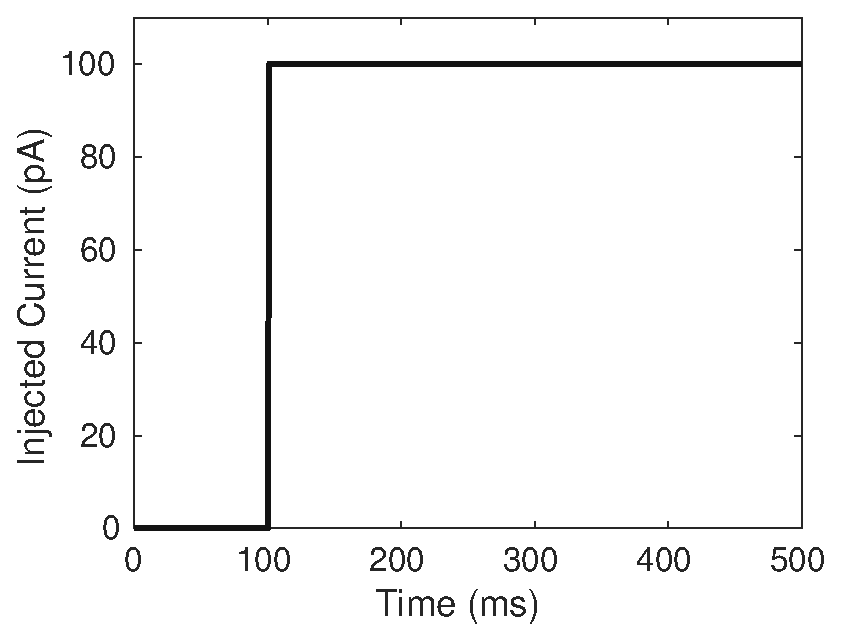
\includegraphics[width=0.8\linewidth]{InjectedCurrent.eps}
            }&
            \sidesubfloat[]{\label{fig:membrane_response_baseline}
                \centering
                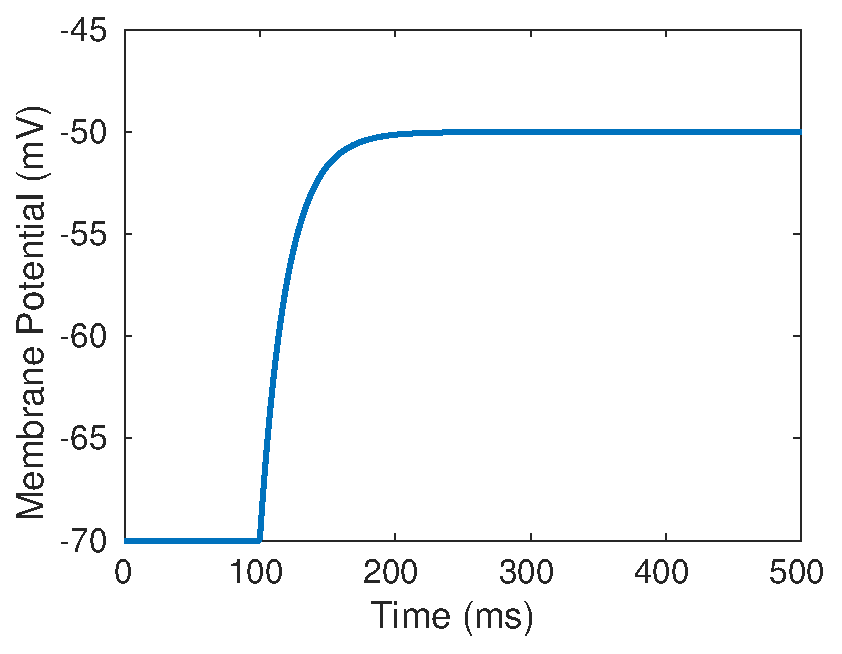
\includegraphics[width=0.8\linewidth]{MembranePotential_Baseline.eps}
            }
        \end{tabular}
        \caption{\label{fig:membrane_dynamics_simulation}
        Simulation of membrane dynamics using \cref{eqn:membrane_voltage_with_current}.
        \protect\subref{fig:injected_current} Injected current
        \protect\subref{fig:membrane_response_baseline} Membrane potential}.
    \end{figure}
    \cref{fig:membrane_dynamics_simulation} shows the simulation results for membrane potential for an input current $I_{s}(t)$ shown in \cref{fig:injected_current}.
    The membrane voltage $V_{m}(t)$ in response to the current is shown in \cref{fig:membrane_response_baseline}.

    In \cref{fig:cg_variation}, we simulate the membrane equation with different choices of the model parameters.
    \cref{fig:varying_membrane_capacitance} shows the membrane dynamics over a range of capacitance values.
    Since the time constant $\tau$ can be expressed as $\frac{C}{G_{leak}}$, reducing membrane capacitance reduces the time-constant, which in turn results in faster dynamics.
    We can observe that for $C=200pF$, it take longer to charge the membrane capacitance to it final value when compared to a smaller capacitance value (say $C=10pF$).
    Additionally, we observe that the steady-state membrane voltage (in the presence of injected current), is independent of the capacitance value.

    \begin{figure}[H]
        \begin{tabular}{p{0.3\textwidth}p{0.3\textwidth}p{0.3\textwidth}}
            \sidesubfloat[]{\label{fig:varying_membrane_capacitance}
                \centering
                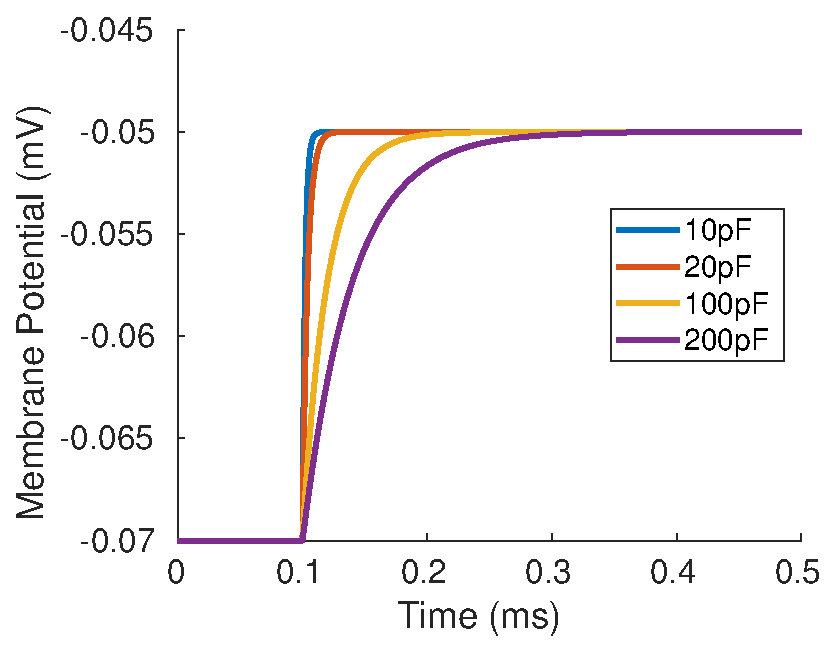
\includegraphics[width=0.8\linewidth]{VaryingMembraneCapacitance.eps}
            }&
            \sidesubfloat[]{\label{fig:varying_leakage_conductance}
                \centering
                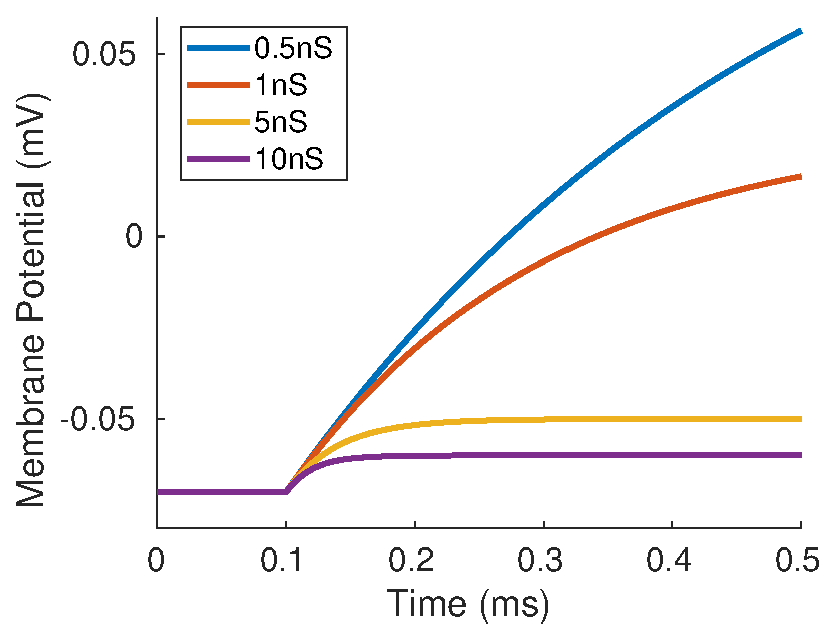
\includegraphics[width=0.8\linewidth]{VaryingLeakageConductance.eps}
            }&
            \sidesubfloat[]{\label{fig:preseving_tau_in_variation}
                \centering
                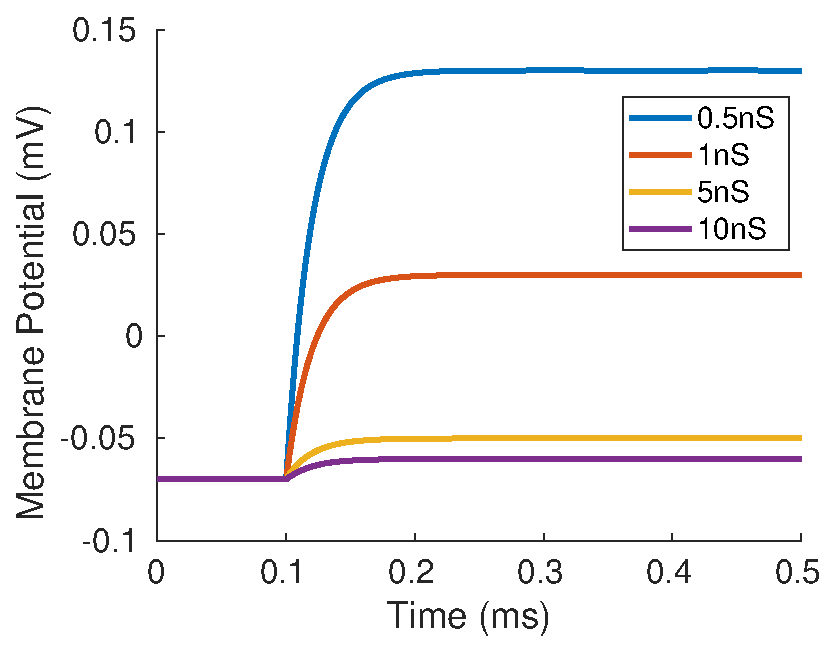
\includegraphics[width=0.8\linewidth]{TauPreservingGleakVariance.eps}
            }
        \end{tabular}
        \caption{\label{fig:cg_variation}
        Varying membrane parameters and analyzing the effect on voltage dynamics.
        \protect\subref{fig:varying_membrane_capacitance} Varying membrane capacitance with fixed leakage conductance $G_{leak}$ ($5nS$).
        \protect\subref{fig:varying_leakage_conductance} Varying leakage conductance with fixed membrane capacitance $C$ ($100pF$).
        \protect\subref{fig:preseving_tau_in_variation} Simultaneous variation of $C$ and $G_{leak}$ such that the time constant $\tau=\frac{C}{G_{leak}}$ is preserved.
        }
    \end{figure}
    When we vary the leakage conductance $G_{leak}$, in \cref{fig:varying_leakage_conductance}, we observe that the steady state membrane potential changes.
    A lower value of $G_{leak}$ leads to a higher steady state membrane potential.
    In steady state, the membrane potential is related to the leakage conductance as $G_{leak}(V_{m} - V_{r}) = I_{s}$, giving us an inverse relationship between $V_{m}$ and $G_{leak}$.
    Furthermore, the time constant for charging the membrane potential increases as we decrease $G_{leak}$, slowing down the membrane dynamics as we decrease $G_{leak}$.

    We can also vary $C$ and $G_{leak}$ together, such that their ratio ($\tau$) is preserved.
    As shown in \cref{fig:preseving_tau_in_variation}, in this case, it takes the same amount of time to charge the cell membrane to its final value.
    However, the steady-state membrane potential decreases as we increase $G_{leak}$, as we observed earlier in \cref{fig:varying_leakage_conductance}.

    \begin{figure}[H]
        \begin{tabular}{p{0.45\textwidth}p{0.45\textwidth}}
            \sidesubfloat[]{\label{fig:Na_K_sweep}
                \centering
                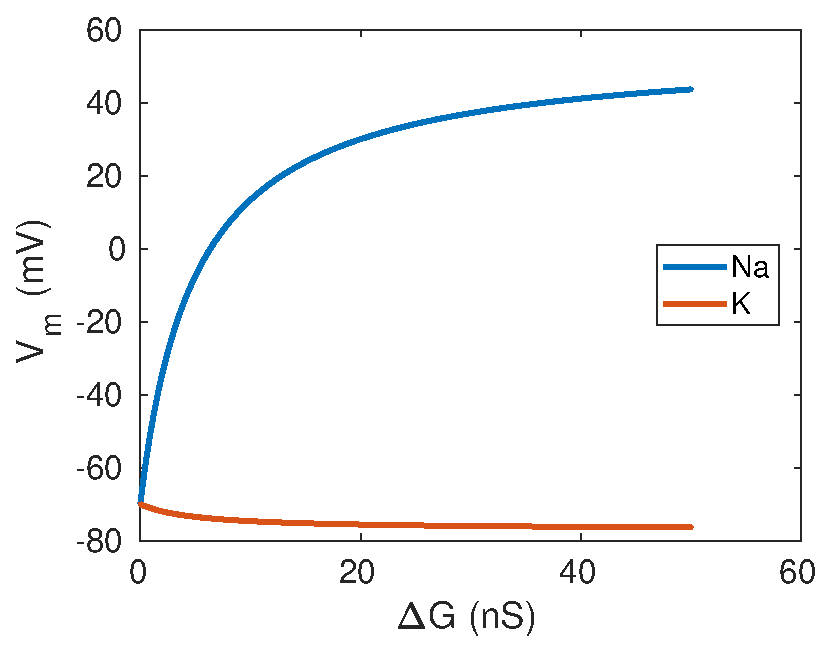
\includegraphics[width=0.8\linewidth]{SynapticInputs_KandNa.eps}
            }&
            \sidesubfloat[]{\label{fig:shunting_inhbition}
                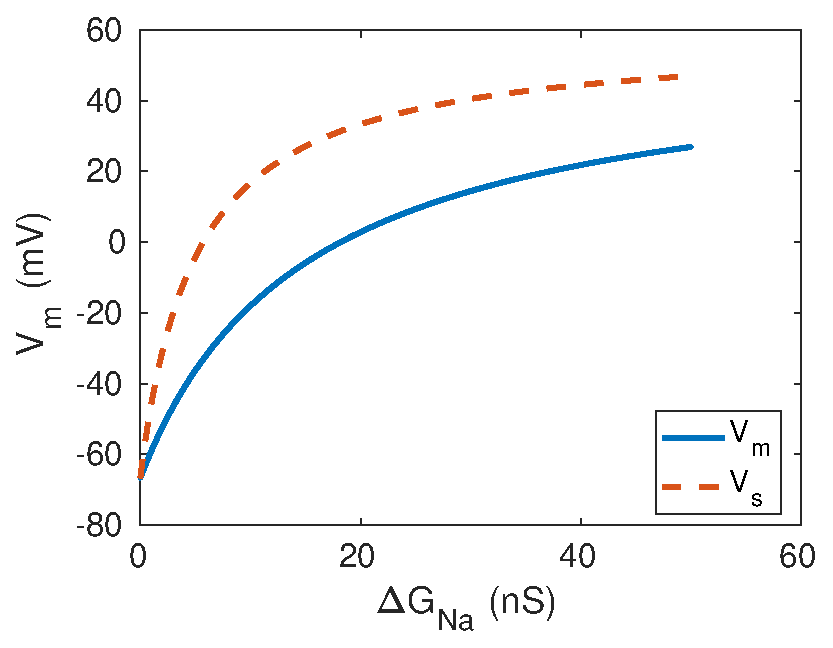
\includegraphics[width=0.8\linewidth]{SynapticInputs_Cl.eps}
            }
        \end{tabular}
        \caption{\label{fig:synaptic_inputs}
        Role of synaptic input in membrane excitability
        \protect\subref{fig:Na_K_sweep} Sweeping Sodium ($Na^+$) and Potassium ($K^+$) conductance and measuring steady-state membrane potential ($V_{m}$).
        \protect\subref{fig:shunting_inhbition} Measuring steady-state membrane potential $V_{m}$ as we sweep $G_{Na}$ with Chloride $Cl^{-}$ conductance increased by $10nS$.
        $V_{s}$ (dotted) showing the superposition of contribution from $Cl^{-}$ and $Na^+$ conductance individually.
        }
    \end{figure}

    In \cref{fig:synaptic_inputs}, we explore the role of synaptic transmission in the excitability of the cell membrane.
    \cref{fig:Na_K_sweep} shows the steady state membrane potential as we sweep the Sodium ($Na^+$) and Potassium ($K^+$) conductance between $0nS$ and $50nS$.
    The reversal potentials for $Na^+$ and $K^+$ are $55$mV and $-77$mV respectively.
    At higher values of conductances, $Na^+$ and $K^+$ drive the steady state membrane voltage to their respective reversal potentials.

    We also explore the role of $Cl^-$ in \cref{fig:shunting_inhbition}.
    If we increase $Cl^-$ conductance by $10$nS ($\Delta{G_{Cl}}=10nS$), we observe a change in the response of steady state membrane potential with respect to sodium conductance ($\Delta{G_{Na}}$).
    Interestingly, this change in response is more than what we would expect from a linear superposition of the contributions of $Cl^-$ and $Na^+$ as shown in \cref{fig:shunting_inhbition} (dotted line, $V_{s}$).

    We can express the steady-state membrane potential $V_{m,ss}$ by rewriting \cref{eqn:membrane_voltage_no_current} as
    \begin{align}
        V_{m,ss} &= \frac{V_{r}G_{leak} + V_{Na}\Delta{G_{Na}} + V_{Cl}\Delta{G_{Cl}}}{G_{leak} + \Delta{G_{Na}} + \Delta{G_{Cl}}}.
        \label{eqn:steady_state_membrane_potential}
    \end{align}
    Here, we have assumed that $\Delta{G_{K}}=0$ and only the synaptic input from $Na^+$ and $Cl^-$ channels drives the membrane's steady state.
    In the steady-state formulation, $\Delta{G_{Cl}}$ appears in both the numerator and denominator in \cref{eqn:steady_state_membrane_potential}, and therefore, it non-linearly nullifies the effect of $Na^+$ contribution to lower the membrane's excitability.
    The primary driver of this non-linearity is the contribution of $\Delta{G_{Cl}}$ to $G_{total}$ in the denominator of \cref{eqn:steady_state_membrane_potential}.

    $Cl^-$ conductance, therefore, plays an interesting, non-linear role in modulating the response of the cell.
    By activating $Cl-$ channels via GABAergic synapses, the overall excitability is reduced\footnote{Excitation of the cell membrane leads to depolarization which in turn is hindered by the activation of $Cl-$ channels.}.

    \section{Appendix: Code}
    \label{sec:appendix_code}

    \begin{center}
        \begin{minipage}{0.9\textwidth}
            \lstinputlisting[caption=Matlab Code for Membrane model\label{lst:membrane_model}]{membrane_model.m}
        \end{minipage}
    \end{center}

    \begin{center}
        \begin{minipage}{0.9\textwidth}
            \lstinputlisting[caption=Matlab Code for simulating the Membrane model as an ODE\label{lst:membrane_simulation}]{membrane_simulation.m}
        \end{minipage}
    \end{center}

    \begin{center}
        \begin{minipage}{0.9\textwidth}
            \lstinputlisting[caption=Matlab Code for steady-state analysis of Membrane potential and contribution of synaptic inputs\label{lst:synaptic_inputs}]{synaptic_inputs.m}
        \end{minipage}
    \end{center}
\end{document}
